In Section~\ref{sec:language}, we said that the SSSP program has an optimal
scheduling if the nodes with the shortest distances are selected to run before
other nodes.  The coordinated version of the SSSP
program is presented in Fig.~\ref{code:shortest_path_program_coord} and it
uses one coordination fact, namely \texttt{set-priority} (line 14). Note that we
also use a global program directive to order priorities in ascending order (line
5).

When using a single thread, the algorithm behaves like
Dijkstra's shortest path algorithm~\cite{Dijkstra}. However, when using multiple
threads, each thread will pick the smallest distance from their subset of nodes.
While this does not yield the optimal program with relation to 1 thread, it
allows for parallel execution and locally avoid unnecessary work. XXX

\begin{figure}[h!]
\scriptsize\begin{Verbatim}[numbers=left,commandchars=\\\{\}]
type route edge(node, node, int).
type linear shortest(node, int, list int).
type linear relax(node, int, list int).

\underline{priority @order asc}.

shortest(A, +00, []).
relax(@1, 0, [@1]).

shortest(A, D1, P1), D1 > D2, relax(A, D2, P2)
   -o shortest(A, D2, P2),
      \{B, W | !edge(A, B, W) |
         relax(B, D2 + W, P2 ++ [B]),
         \underline{set-priority(B, float(D2 + W))}\}.

shortest(A, D1, P1), D1 <= D2, relax(A, D2, P2)
   -o shortest(A, D1, P1).
\end{Verbatim}
  \caption{Shortest Path Program.}
  \label{code:shortest_path_program_coord}
\end{figure}
\normalsize

The most interesting property of the SSSP program presented in
Fig.~\ref{code:shortest_path_program_coord} is that it remains provably correct,
although it applies rules using smarter ordering. The derivation of
\texttt{set-priority} does not change the behavior of the logical rules and the
code remains declarative.

Figure~\ref{results:sssp_uspowergrid} shows experimental results a
SSSP program that computes the SSSP for 20\% of the nodes of the graph.
There are some situations where unecessary facts are propagated
because although the shortest distance is selected, sub-optimal distances may be
propagated because many SSSP distances are computed at the same time.
However, we see a reduction of over 50\% in the number of
derived facts when using the coordinated version \textbf{C} over the regular
version \textbf{R}. The results also show that the cordinated
version using 16 threads is 1.3 times faster than the regular version using 16
threads. In turn, this makes the coordinated version 20 times faster
than the regular version using 1 thread. Note that the coordinated program is as
scalable as the regular program.

\begin{figure}[h!]
   \begin{center}
      \subfloat[]{ \begin{tabular}[b]{ | c | c | c | }
         \hline                       
         \textbf{\# T} & \textbf{R} & \textbf{C} \\ \hline \hline
         1 & 333K & 206K \\
         2 & 300K & 210K \\
         4 & 316K & 208K \\
         8 & 328K & 211K \\
         16 & 343K & 212K \\
         \hline  
         \end{tabular}
         \normalsize
      }
      \subfloat[]{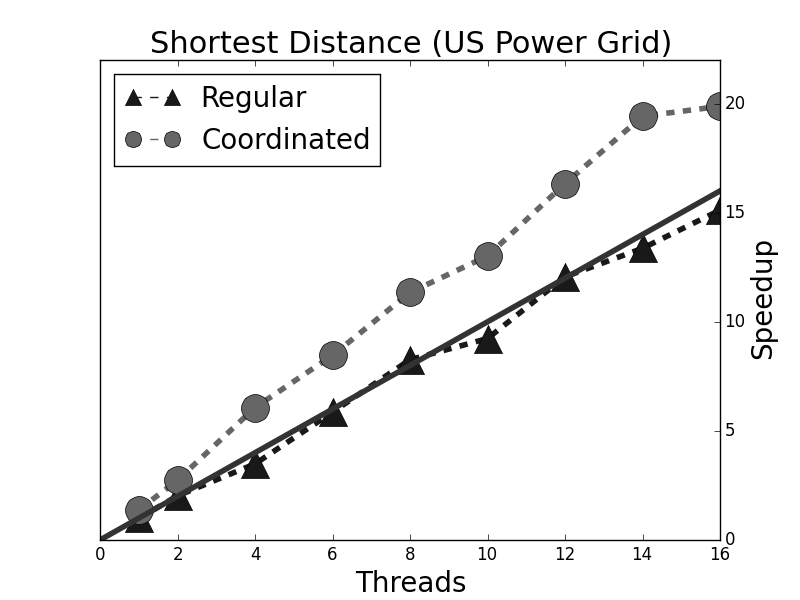
\includegraphics[width=5.5cm]{results/shortest-uspowergrid.png}}
   \end{center}
   \caption{Experimental results for the SSSP program using US powergrid network.
   On the left we show the number of facts derived for the regular \textbf{R}
   and coordinated version \textbf{C} using a variable number of threads
   \textbf{\# T}. On the right, we have the scalability of the regular and
   coordinated version. The speedup values are computed using the execution
   time for 1 thread.}
   \label{results:sssp_uspowergrid}
\end{figure}
